\documentclass[12pt, a4paper]{article}
\usepackage [utf8]{inputenc}
\usepackage [portuges]{babel}
\usepackage {graphicx}
\usepackage {enumerate}
\usepackage {color}

\title{\Huge{\textsf{\textbf{Projeto de LI1}}} - \textit{LightBot}}

 
\author{\large{\emph{João Coelho A74859}} \and \large{\emph{Fábio Baião A75662}}} 


\large{\date{\textrm{\today}}}

\begin{document}

\maketitle

\begin{figure}[h]
\centering
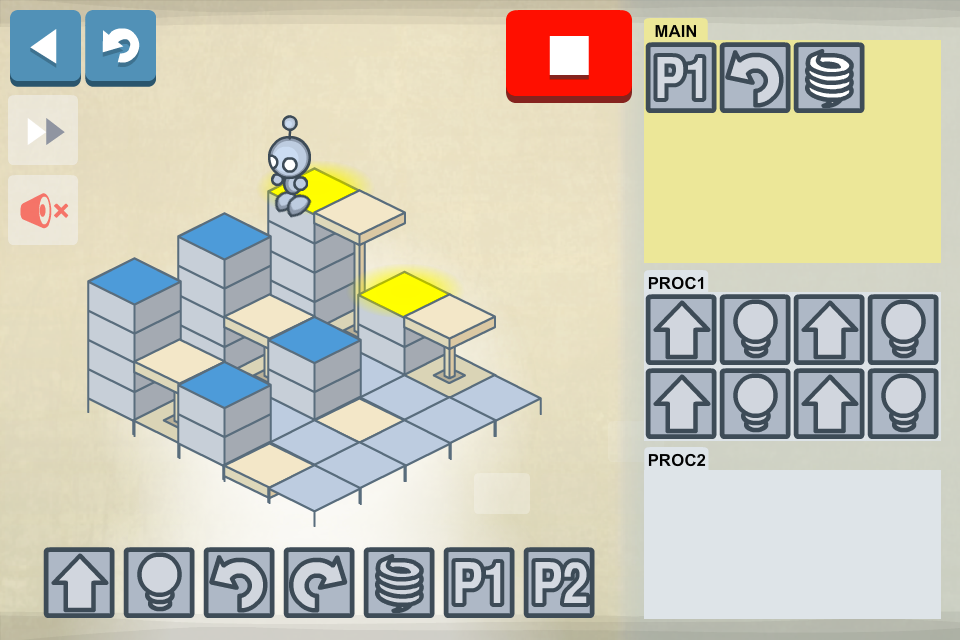
\includegraphics[scale=0.45]{./unnamed.png}
\textbf{\caption{Tabuleiro do jogo \textit{LightBot}}}
\end{figure}

\newpage

\tableofcontents

\newpage 

\section{Introdução ao Projeto}

% aqui será feita uma apresentação do projeto desenvolvido, com referências ao jogo que se pretende criar e restantes objetivos

\subsection{\textit{LightBot}}
% breve apresentação do jogo
 
\begin{itemize}
\item O projeto baseia-se na criação de um jogo virtual à semelhança do puzzle \textit{LightBot}, onde se controla um \textit{robot} num tabuleiro de blocos, com recurso a comandos muitos simples, com vista a acender todas as lâmpadas disponíveis.
\item Consoante o nível, o jogador depara-se com um novo tabuleiro, com nível de dificuldade de resolução crescente, isto é, com lâmpadas cuja localização se torna progressivamente mais desafiante alcançar. 
\item Este projeto é constituído por duas fases com diferentes tarefas.
\end{itemize}

\subsection{Objetivos do grupo}
% criar o nosso primeiro jogo é sempre marcante para estudantes de Eng Informática

\begin{itemize}
\item Este projeto de LI1 proporcionar-nos-á a criação do nosso primeiro jogo, algo que é sempre marcante para estudantes de Engenharia Informática. Como tal, esperamos conseguir neste projeto ser criativos, tendo em vista não só uma melhor classificação como também a gratificação pelo trabalho realizado quando terminada a criação do jogo.  
\item Por outro lado, e não menosprezando a avaliação, pensamos que a satisfação pessoal é também relevante aquando da realização de um projeto, pelo que um dos nosso objetivos estipulados é precisamente desfrutarmos da criação deste jogo. 
\end{itemize}

\subsection{Especificações globais - Entrada/Saída de Dados}

\begin{itemize}
\item O \underline{\textbf{formato de entrada}} é essencialmente comum a todas as tarefas (com uma pequena exceção na tarefa 4), representando o tabuleiro onde o \textit{robot} se move, para além da sua posição e orientação inicial e do programa para o controlar. Por exemplo, \\

aacdD \\
aacaa \\
bbCaa \\
0 1 S \\
SEASLEAADSAL \\

onde as três primeiras linhas correspondem a um tabuleiro representado por 3 linhas, cada uma delas com 5 caracteres alfabéticos, os quais estão associados a diferentes níveis de altura (o carácter \textbf{a} ou \textbf{A} corresponde ao nível 0, o \textbf{b} ou \textbf{B} ao 1 e assim sucessivamente). Note-se ainda que a colocação de letra maiúscula ocorre apenas se a posição tem uma "lâmpada"; a linha seguinte dá-nos a informação relativa às coordenadas x e y, respetivamente, da posição inicial do robot, bem como a sua orientação (N, S, E ou O); a linha final são os comandos que definem a movimentação do \textit{robot} no tabuleiro, variando entre A (avançar), S (saltar), E (esquerda), D (direita) e L (luz).

\item O \underline{\textbf{formato de saída}}, contrariamente ao de entrada, é específico para cada uma das tarefas.
\end{itemize}

\section{Tarefa 1}
% informação referente à primeira tarefa

\begin{enumerate}
    \item O objetivo desta primeira tarefa passava pela criação de um programa que validasse se o \textit{input} fornecido cumpria os requisitos impostos pelo formato de entrada. Após verificar se as linhas do tabuleiro possuíam o mesmo tamanho, se a linha das coordenadas da posição inicial apresentava a estrutura devida e se os comandos eram válidos, o respetivo programa deveria imprimir "OK", se o formato do \textit{input} estivesse de acordo com o estabelecido, ou o número da linha em que primeiramente os dados divergiram do formato prescrito.

\begin{figure}[h]
\centering
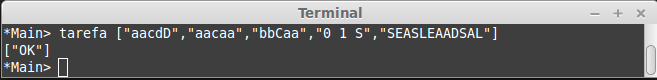
\includegraphics[scale=0.65]{./1.png}
\textbf{\caption{Resposta impressa quando o \textit{input} é válido}}
\end{figure}    
    
    \item Para solucionar o problema, criou-se um programa suportado essencialmente em seis funções auxiliares:

\begin{enumerate} [i.]
    \item Duas responsáveis por verificar a validade do tabuleiro, ou seja, se as linhas têm o mesmo tamanho.
   
\begin{figure}[h]
\centering
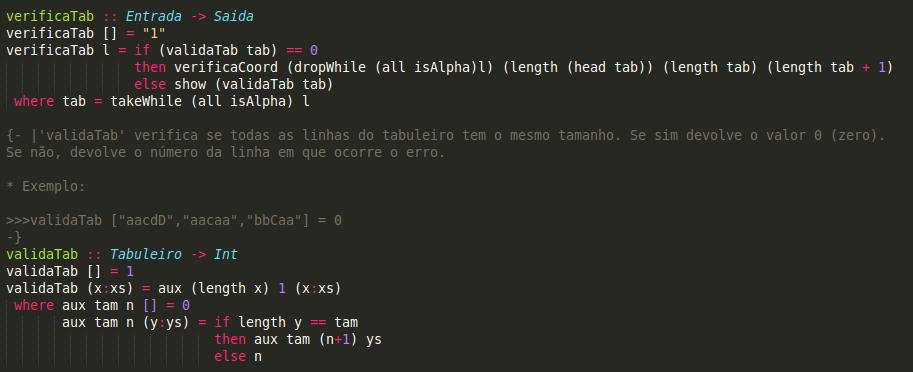
\includegraphics[scale=0.45]{./2.png}
\textbf{\caption{Funções auxiliares que verificam se o tabuleiro é válido}}
\end{figure}    

\newpage 

    \item Outras duas que testam a validade da posição inicial, verificando se as coordenadas são maiores ou iguais que 0 e menores que o tamanho do tabuleiro e se a orientação respeita a prescrição do formato de entrada. 
    
\begin{figure}[h]
\centering
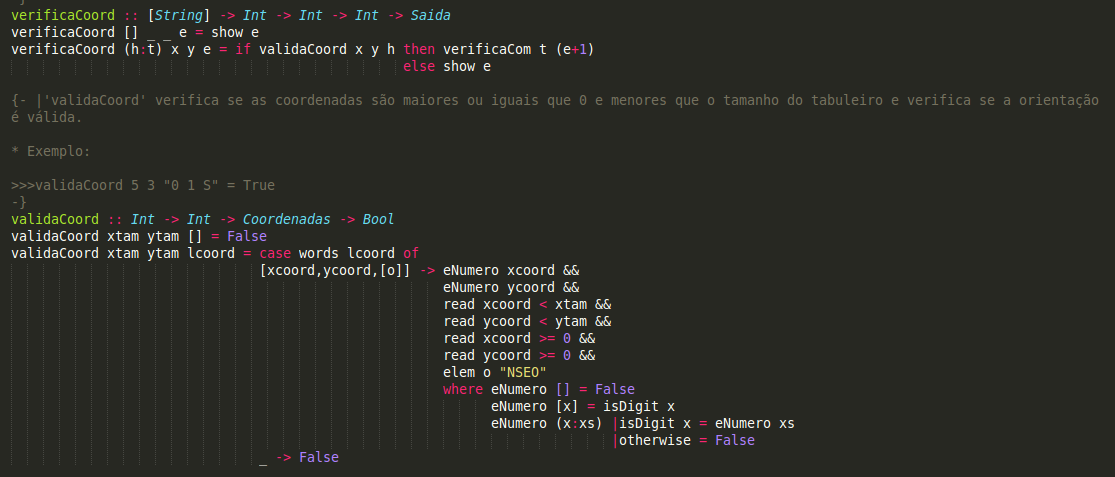
\includegraphics[scale=0.40]{./3.png}
\textbf{\caption{Funções auxiliares que verificam a validade da linha das coordenadas da posição inicial}}
\end{figure}    

    





    \item E ainda duas outras que atuam sobre a(s) última(s) linha(s) do \textit{input}: uma que verifica a validade dos comandos, retornando o número da linha que os inclui se não forem válidos, e outra que, no caso de estes serem válidos, verifica se não existe mais nada em baixo, devolvendo o número da linha abaixo da linha de comandos se existir ou "OK" se não. É, portanto, nesta fase que o programa devolve "OK" em caso de o \textit{input} ser aprovado, já que a aprovação na verificação dos comandos pressupõe que as prescrições anteriores impostas pelo formato de entrada foram respeitadas.   

\begin{figure}[h]
\centering
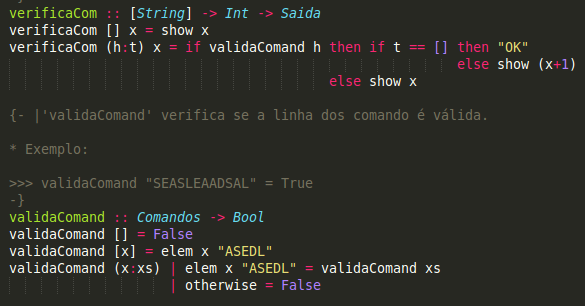
\includegraphics[scale=0.50]{./4.png}
\textbf{\caption{Funções auxiliares que testam a linha de comandos}}
\end{figure}    

\end{enumerate}
    
    \item Nesta tarefa, o objetivo traçado pelo Projeto foi alcançado na plenitude pelo grupo, obtendo a classificação máxima de pontos na avaliação do \textit{Mooshak}. É de referir também que, associados a esta primeira tarefa, foram realizados e aprovados mais de trinta testes,contendo cada um deles um \textit{input} diferente, com o intuito de pôr a prova o programa criado. Note-se que os testes são não mais do que uma simulação da funcionalidade do programa, logo em qualquer tarefa passam pela criação de um ficheiro com o \textit{input} e outro com o respetivo \textit{output}, estando a aprovação no teste dependente de o \textit{output} manualmente criado coincidir com o ficheiro resultado dado pela \textit{Makefile}. 
\end{enumerate}  

\section{Tarefa 2}
% informação referente à segunda tarefa

\begin{enumerate}
    \item No que à segunda tarefa diz respeito, o Projeto apresentava como objetivo a implementação de um programa que determinasse a posição do \textit{robot} após a execução do primeiro comando, fornecido por um \textit{input} que se assumia estar de acordo com as especificações estipuladas pelo formato de entrada. Após identificar qual o primeiro comando, o respetivo programa deveria retornar "ERRO" no caso do comando não ser aplicável (por exemplo, comando L sobre uma posição do tabuleiro sem \textit{lâmpada} ou comando S quando o nível da posição final é superior em mais de uma unidade em relação ao da posição inicial)ou, sendo aplicável, deveria apresentar a posição seguinte do \textit{robot} de forma análoga à linha da posição inicial. 

\begin{figure}[h]
\centering
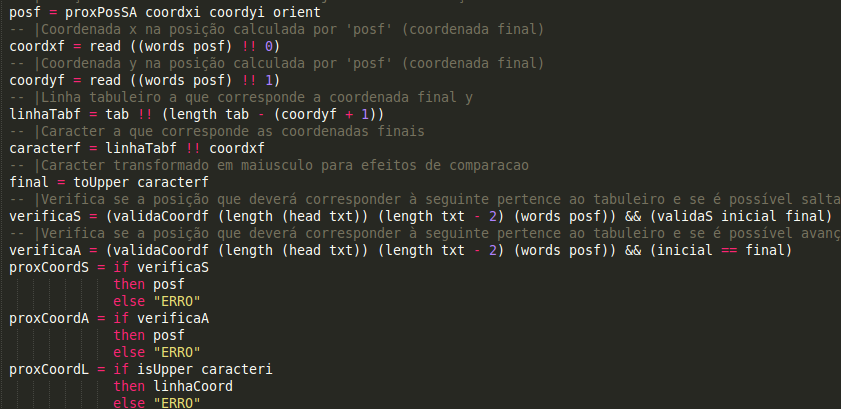
\includegraphics[scale=0.50]{./5.png}
\textbf{\caption{Evidência de como o programa obedece às exigências formais da tarefa}}
\end{figure}  


    \item Este novo programa, respeitando o estipulado, inicialmente encontra o primeiro comando. Em seguida, ocorre a verificação da aplicabilidade desse comando: 
  
\begin{enumerate} [i.]
     \item A verificação dos comandos S e A acarretam um grau de dificuldade acrescido, dado ser necessário, em primeiro lugar, verificar se a posição seguinte pertence ao tabuleiro e depois comparar os níveis das duas posições, sendo que: só é possível saltar se o nível da posição inicial for superior ao da final ou inferior em um nível apenas; só é aplicável o A se o nível das duas posições for o mesmo.
     
\begin{figure}[h]
\centering
  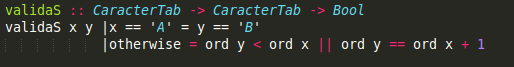
\includegraphics[scale=0.5]{./6.png}
  \textbf{\caption{Função que verifica se é possível saltar}}
\end{figure}











     \item Já a verificação do comando L resume-se a analisar se o carácter que representa a posição inicial no tabuleiro é maiúsculo, uma vez que, como foi anteriormente referido, as posições das lâmpadas são ilustradas no tabuleiro por um carácter maiúsculo. 
     

     \item Quanto aos comandos O e E, a sua aplicabilidade é universal, logo o programa ignora a verificação e devolve de imediato as coordenadas da posição final.

\begin{figure}[h]
  \centering
  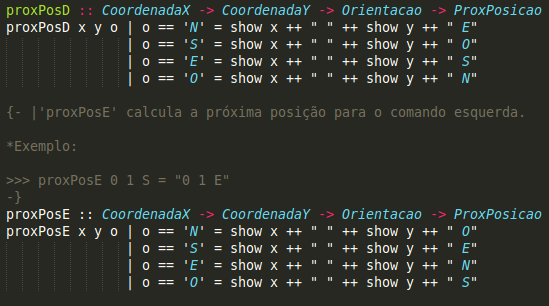
\includegraphics[scale=0.5]{./9.png}
  \textbf{\caption{Função que calcula a próxima posição para O e E}}
\end{figure}





\end{enumerate}



   \item Para os diferentes comandos segue-se: 
\begin{enumerate} [i.]
     \item Após a verificação, para S e A, se a posição final pertencer ao tabuleiro, a função verifica se é possível saltar e avançar, respetivamente. Caso seja possível, o programa devolve a posição final já calculada, senão retorna "ERRO".

\begin{figure}[h]
  \centering
  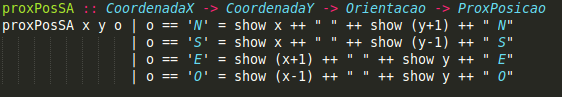
\includegraphics[scale=0.45]{./7.png}
  \textbf{\caption{Função que calcula a próxima posição para S e A}}
\end{figure}     









     \item Para L, caso se confirme a validade deste comando, a próxima posição será coincidente com a posição inicial.
  \begin{figure}[h]
  \centering
  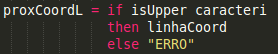
\includegraphics[scale=0.5]{./8.png}
  \textbf{\caption{Função que devolve a linha das coordenadas da posição inicial se o carácter for maiúsculo}}
\end{figure}
   






     \item As coordenadas da posição final, se o comando inicial for E ou O, divergirão das da inicial apenas na parecela referente à orientação.
\end{enumerate}

  \item Nesta segunda tarefa, foi também possível ao grupo obter pontuação máxima na avaliação levada a cabo pelo \textit{Mooshak}, o que demonstra que foram cumpridos os objetivos definidos pelo enunciado do Projeto para esta tarefa, algo passível de se concluir também pelo facto de os testes realizados para esta segunda etapa do trabalho terem recebido na totalidade resposta positiva.
\end{enumerate}

\section{Tarefa 3}
% informação referente à terceira tarefa

\begin{enumerate}
    \item A tarefa 3, última desta primeira fase do Projeto, requeria um programa capaz de fazer o \textit{robot} executar a sequência de comandos, fornecida pelo \textit{input}, até acender todas as lâmpadas disponíveis. Novamente, assumia-se que o \textit{input} estaria de acordo com as prescrições do formato de entrada. Considerando que os comandos eram executados em sequência e que aqueles que não fossem aplicáveis deveriam deixar o estado do \textit{robot} inalterado, ao programa criado era exigido que imprimisse uma linha contendo as coordenadas "x" e "y" da posição do \textit{robot} no momento (separadas por um único espaço), sempre que um comando L fosse executado com sucesso. Se todas as \textit{lâmpadas} do tabuleiro fossem acesas, o programa deveria terminar, independentemente da existência de comandos não executados, retornando a mensagem "FIM «Num»", sendo «Num» o número de comandos válidos executados. Caso contrário, se a sequência de comandos terminasse sem que todas as \textit{lâmpadas} se encontrassem acesas, deveria imprimir "INCOMPLETO".  
    
\begin{figure}[h]
  \centering
  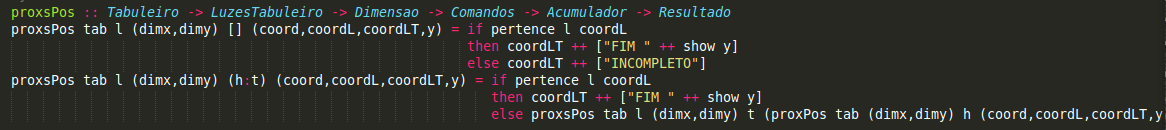
\includegraphics[scale=0.35]{./10.png}
  \textbf{\caption{Programa retorna FIM «Num» ou INCOMPLETO como é suposto}}
\end{figure}    





    \item O funcionamento do programa criado pelo grupo para dar resposta ao problema colocado por esta terceira tarefa baseia-se em:

\begin{enumerate} [i.]
    \item Calcular sucessivamente a próxima posição dependendo do comando a executar, pelo que parcelas do programa da tarefa anterior são aplicadas também nesta. Dado que, para efeito dos dados finais devolvidos pelo programa, é necessário contabilizar os comandos executados, foi adicionado um acumulador à função que calcula a próxima posição, que aumenta uma unidade sempre que um comando seja aplicável.  
 \begin{figure}[h]
  \centering
  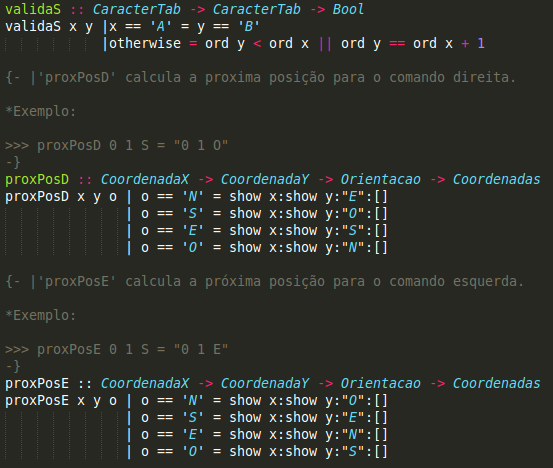
\includegraphics[scale=0.5]{./11.png}
  \textbf{\caption{Algumas funções comuns à tarefa anterior}}
\end{figure} 


















\begin{figure}[h]
  \centering
  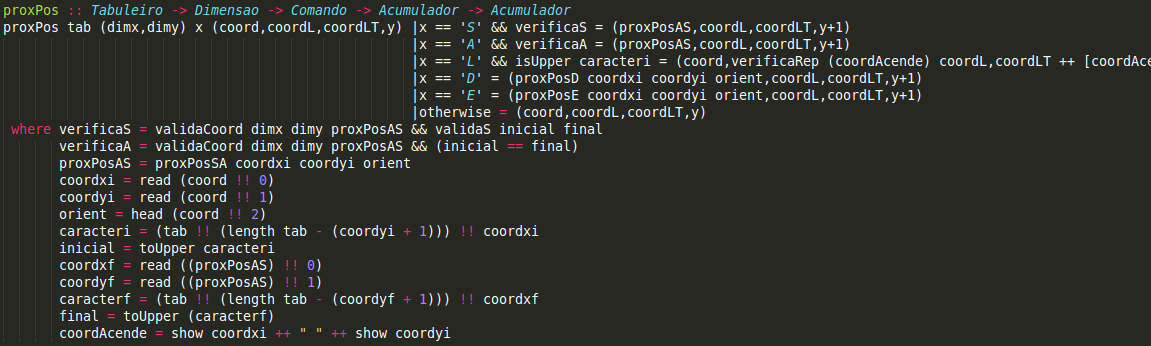
\includegraphics[scale=0.35]{./12.png}
  \textbf{\caption{Função com acumulador mencionada em i.}}
\end{figure} 















    \item Todavia, antes de calcular a posição seguinte há uma verificação se as \textit{lâmpadas} estão todas acesas. Caso estejam, o programa termina e imprime o resultado final, dentro das características do output para a terceira tarefa.
    

    \item É também de mencionar o modo como o programa atua sobre as listas das coordenadas das \textit{lâmpadas}. As três primeiras funções apresentadas na figura 14 calculam a lista das onde existe \textit{lâmpada},ou seja, carácter maiúsculo no tabuleiro. À medida que o \textit{robot} acende as \textit{lâmpadas}, as coordenadas das que já estão acesas são guardadas numa lista, porém sempre que o \textit{robot} executa o comando L nas coordenadas de uma \textit{lâmpada} já acesa, ela é apagada e essas coordenadas são removidas da lista. Se o comando L voltar a ser executado nessa coordenadas, elas são reintroduzidas na lista. Para salvaguardar isto, foi necessário criar uma função que verificasse se as coordenadas onde foi executado com sucesso o comando L já existiam na lista só com as coordenadas de \textit{lâmpadas} acesas. É esta lista, apenas de coordenadas de \textit{lâmpadas} já acesas, que é comparada à que inclui as de todas as \textit{lâmpadas} do tabuleiro, para verificar se foram acesas todas elas.
  \begin{figure}[h]
  \centering
  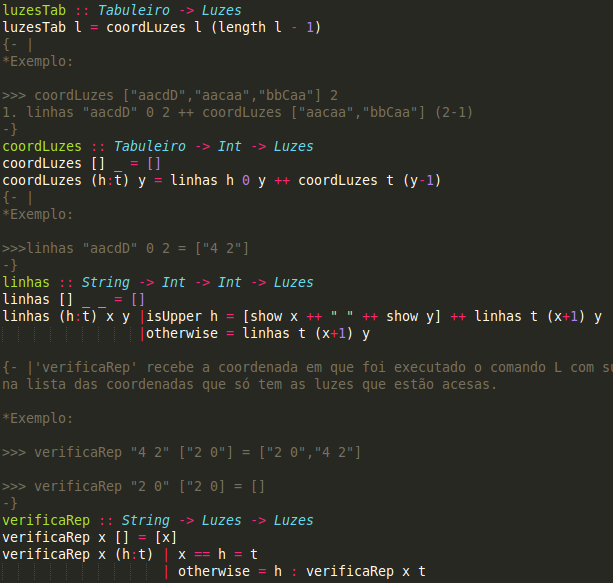
\includegraphics[scale=0.5]{./13.png}
  \textbf{\caption{Funções auxiliares que atuam sobre as coordenadas das \textit{lâmpadas}}}
\end{figure}













\end{enumerate}

\item Essencialmente por questões de eficiência do programa criado, nesta fase a classificação que o \textit{Mooshak} atribuiu ao grupo esteve dois pontos abaixo daquela que era a classificação máxima. Não obstante este facto, os múltiplos ficheiros de teste criados para a tarefa 3 foram aprovados quando corrida a \textit{Makefile}.
\end{enumerate}

\section{Tarefa 4}

\begin{enumerate} 
   \item A tarefa 4 marca o início da segunda fase do Projeto. Nela pretendia-se a realização de um programa que sintetizasse um programa para o \textit{robot} de modo que este conseguisse, a partir da sua posição inicial, acender todas as \textit{lâmpadas} do tabuleiro. Desta forma, era notório que, dependendo do tabuleiro, da posição inicial do \textit{robot} e das posições das \textit{lâmpadas}, a solução para o problema poderia ser simples (quando a diferença de altura, para quaisquer duas posições adjacentes do tabuleiro, fosse de um nível no máximo), complicada (quando nem todos os caminhos entre duas posições do tabuleiro fossem possíveis) ou até mesmo impossível de encontrar (quando existisse pelo menos uma \textit{lâmpada} inalcançável). Tal como nas duas tarefas anteriores, assumia-se que o \textit{input} obedeceria ao formato de entrada estabelecido, com a particularidade de ser omitida a linha referente aos comandos. O \textit{output} esperado corresponderia à linha referente ao programa sintetizado.
  
  \item Para esta tarefa, o programa criado pelo grupo cobre todos os casos simples e boa parte dos complicados. À semelhança da tarefa anterior, é necessário encontrar as coordenadas das posições das \textit{lâmpadas}, pelo que as funções da tarefa 3 responsáveis por esta ação foram reaproveitadas nesta tarefa. No entanto, há diferenças na abordagem a cada uma das situações (casos simples ou complexos): 

\begin{enumerate} [i.]
  \item Uma vez que não existe a necessidade de verificar se é possível ou não ao \textit{robot} saltar, os casos mais simples foram solucionados com recurso a funções que essencialmente atuam sobre a orientação do \textit{robot}, de modo a orientá-lo no caminho até cada \textit{lâmpada}, e selecionam, tanto para os movimentos verticais como horizontais, o comando A (avançar) ou S(saltar), dependendo das posições inicial e final.
 \begin{figure}[h]
  \centering
  \begin{minipage}[b]{0.25\linewidth}
  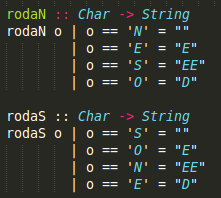
\includegraphics[scale=0.5]{./17.png}
\end{minipage}
\quad
\begin{minipage}[b]{0.65\linewidth}
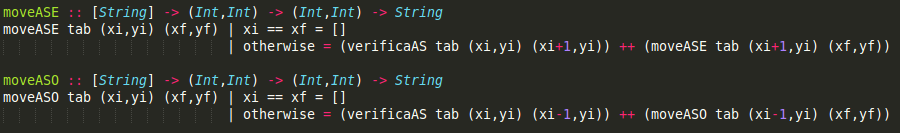
\includegraphics[scale=0.35]{./18.png}
\end{minipage} 
 \textbf{\caption{Algumas das funções que intervêm na orientação do \textit{robot} e na seleção entre os comandos A e S}}
\end{figure}
  


\newpage






  \item Já para os casos mais complexos, foi necessário criar funções auxiliares que, inicialmente, calculam todas as combinações possíveis entre as \textit{lâmpadas}, pois a morfologia do tabuleiro pode não permitir ao \textit{robot} acendê-las pela ordem em que surgem na lista das suas coordenadas, e depois calculam a lista de comandos capaz de acender todas as \textit{lâmpadas} para cada uma das combinações anteriores. 
\begin{figure}[h]
  \centering
  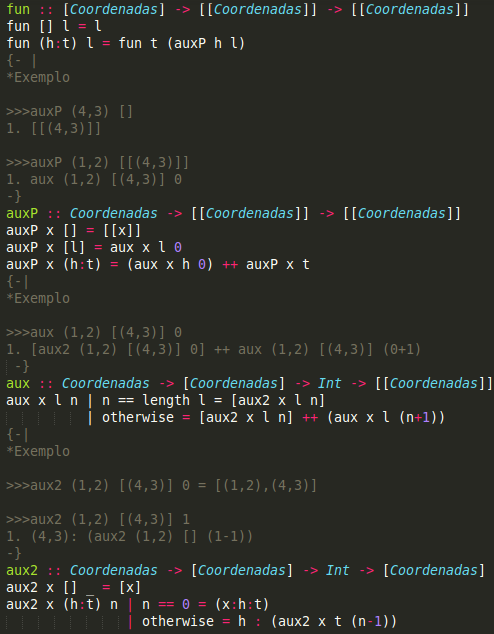
\includegraphics[scale=0.40]{./14.png}
  \textbf{\caption{Funções que calculam todas as combinações possíveis entre as \textit{lâmpadas}}}
\end{figure}






\newpage


  Para o cálculo da lista de comandos, as funções do programa atuam da seguinte forma: testam se, deslocando-se o \textit{robot} primeiro na horizontal e em seguida na vertical (ou vice-versa), este consegue chegar à primeira \textit{lâmpada}. Se sim, avança para a segunda pelo mesmo trajeto (horizontal-vertical ou vice-versa), caso contrário tenta chegar lá pelo trajeto não testado. Esta abordagem é feita para todas as \textit{lâmpadas}, restando porém mencionar que se, na tentativa de alcançar uma delas, nos depararmos com uma situação em que não é possível nem pelo caminho horizontal-vertical nem pelo vertical-horizontal, o programa conclui que a combinação de \textit{lâmpadas} em teste não é possível e passa para o teste da seguinte combinação.
\begin{figure}[h]
  \centering
  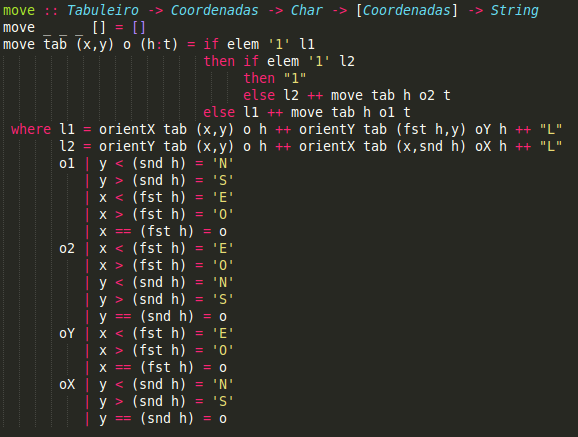
\includegraphics[scale=0.5]{./15.png}
  \textbf{\caption{Função que possibilita a abordagem às \textit{lâmpadas} pelos diferentes trajetos}}
\end{figure}







\newpage

  É também de mencionar que, por uma questão de eficiência, optou-se por, para os casos em que o tabuleiro apresente menos de sete \textit{lâmpadas}, colocar o programa a imprimir como resultado a menor sequência de comandos de entre aquelas obtidas através das diferentes combinações, possíveis, de \textit{lâmpadas}. Para os tabuleiros com mais de sete \textit{lâmpadas}, o programa retorna a lista de comandos derivada da primeira combinação possível. 

\begin{figure}[h]
  \centering
  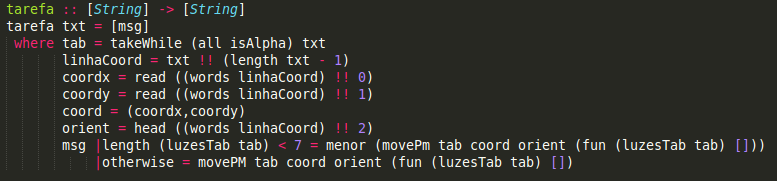
\includegraphics[scale=0.5]{./16.png}
  \textbf{\caption{Evidência do que foi mencionado anteriormente}}
\end{figure}










\end{enumerate}

\item Nesta quarta tarefa, dado que o programa criado não cobre todos os casos mais complexos, o grupo obteve, e há semelhança da classificação atribuída pelo \textit{Mooshak} à tarefa 3, dezoito em vinte pontos totais. Pensa-se que os casos que ficam por cobrir pelo programa referem-se àqueles em que o \textit{robot}, para alcançar uma das \textit{lâmpadas}, necessita de se mover ora na horizontal ora na vertical, alternando sucessivamente. 

\end{enumerate}

\section{Tarefa 5}

\begin{enumerate} 
   \item A tarefa 5 é a segunda tarefa da segunda fase, sendo a última do Projeto. Nela pretendia-se visualizar o jogo criado com recurso ao formato {\large{\emph{X3dom}}}, o qual permite a visualização de cenas tridimensionais em \textit{browsers web}. Como foi dito introdutoriamente, o formato de entrada é comum a todas as tarefas, logo o \textit{input} assemelhar-se-ia aos das tarefas anteriores. Já como \textit{output}, o programa deveria imprimir o código \textbf{xhtml} de uma página web que permitisse visualizar o jogo.
   Dado o carácter subjetivo desta tarefa, os \textit{outputs} poderiam divergir tanto quanto a criatividade dos alunos, pelo que a avaliação seria sempre essencialmente qualitativa.
 
 \item Na quinta tarefa, começou-se por criar o \textit{robot} numa página \textit{html}, explorando o formato {\large{\emph{X3dom}}}, enquanto em simultâneo se geravam as primeiras funções do programa desta tarefa, destinadas à criação de tabuleiros. 
\begin{figure}[h]
  \centering
  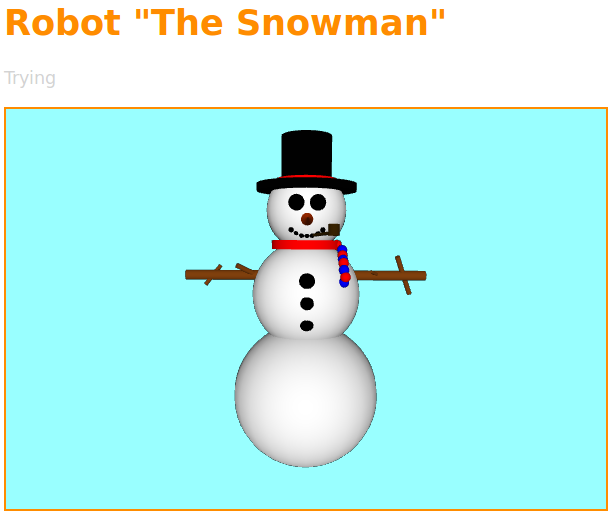
\includegraphics[scale=0.35]{./19.png}
  \textbf{\caption{\textit{Robot}}}
\end{figure}














 Em seguida passou-se às adaptações \textit{html} no programa, necessárias para ser possível, a partir do executável da tarefa e do terminal, obter a visualização do jogo numa página \textit{html}: 


\begin{enumerate} [i.]
  \item Parte destas adaptações passaram por copiar, do enunciado do Projeto para esta tarefa 5, um prefixo e um sufixo comuns a ficheiros \textit{html} deste tipo. 
\begin{figure}[h]
  \centering
  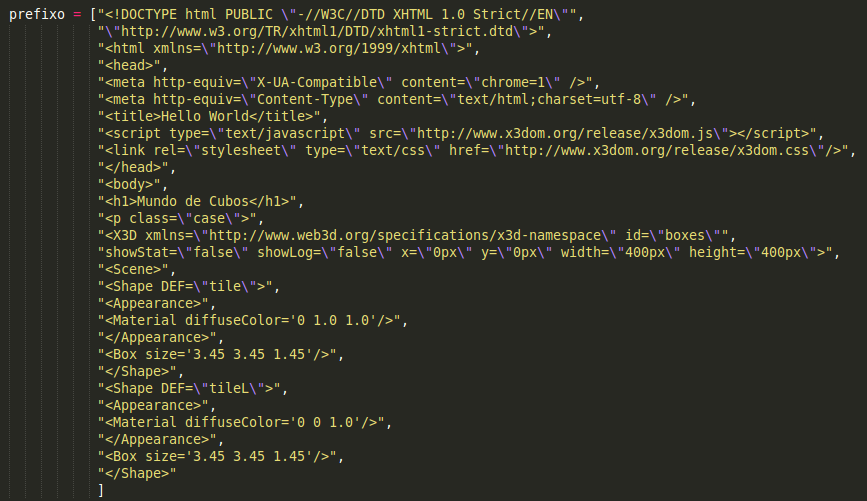
\includegraphics[scale=0.35]{./20.png}
  \textbf{\caption{Prefixo mencionado em i.}}
\end{figure}













  \item Em seguida, para além da criação de funções que permitem colocar o \textit{robot} no tabuleiro fornecido pelo \textit{input}, fizeram-se adaptações \textit{html} às funções que criam os tabuleiros e inseriu-se o código \textit{html} do \textit{robot} no programa sob a forma de sufixo.
\begin{figure}[h]
  \centering
  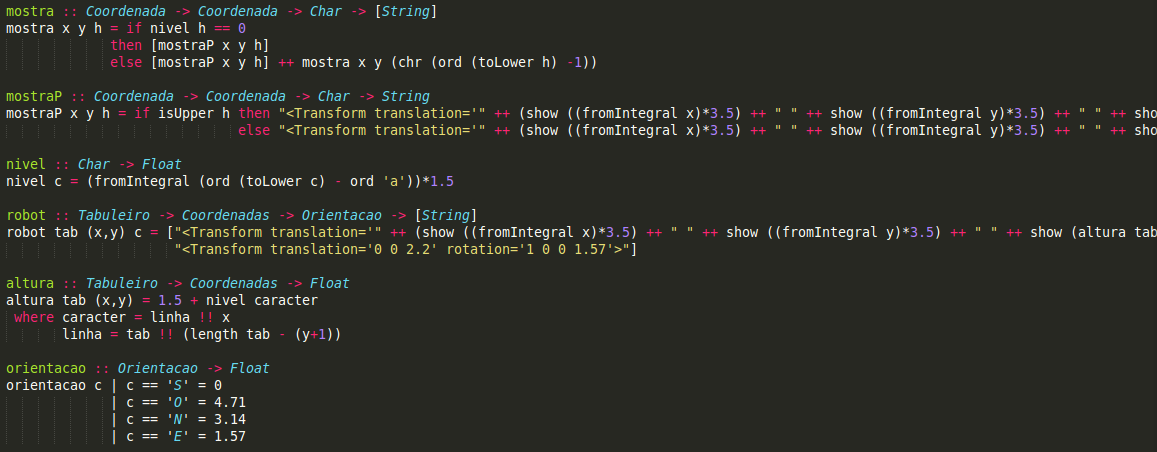
\includegraphics[scale=0.35]{./21.png}
  \textbf{\caption{Adaptações \textit{html}}}
\end{figure}










  \item Por fim, após elaborar num ficheiro \textit{html} a animação do \textit{robot} num tabuleiro específico, procurou-se criar funções \textit{Haskell} que permitam ao programa devolver numa página \textit{html} uma visualização fiel do \textit{robot} a executar os comandos que lhe foram aplicados, isto depois de efetuadas as devidas adaptações. 
\end{enumerate}

\begin{figure}[h]
\centering
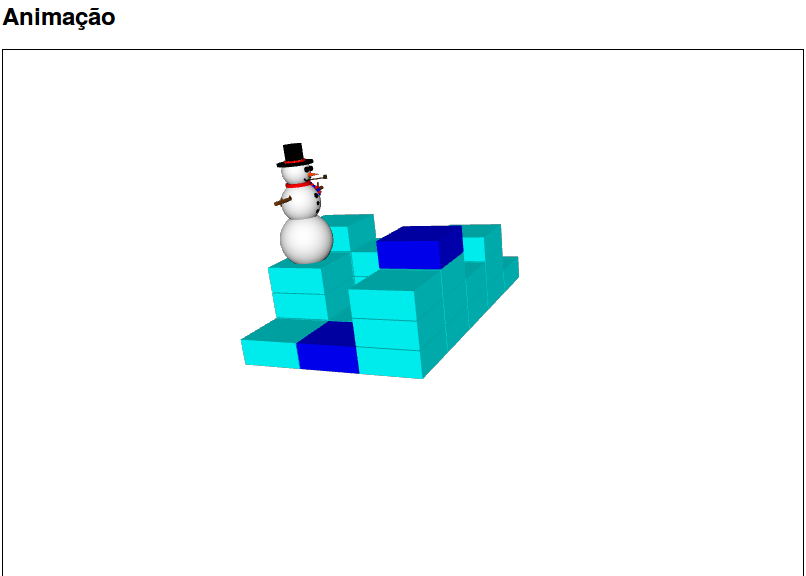
\includegraphics[scale=0.25]{./24.png}
\textbf{\caption{Exemplo de uma animação}}
\end{figure}


\begin{figure}
\centering
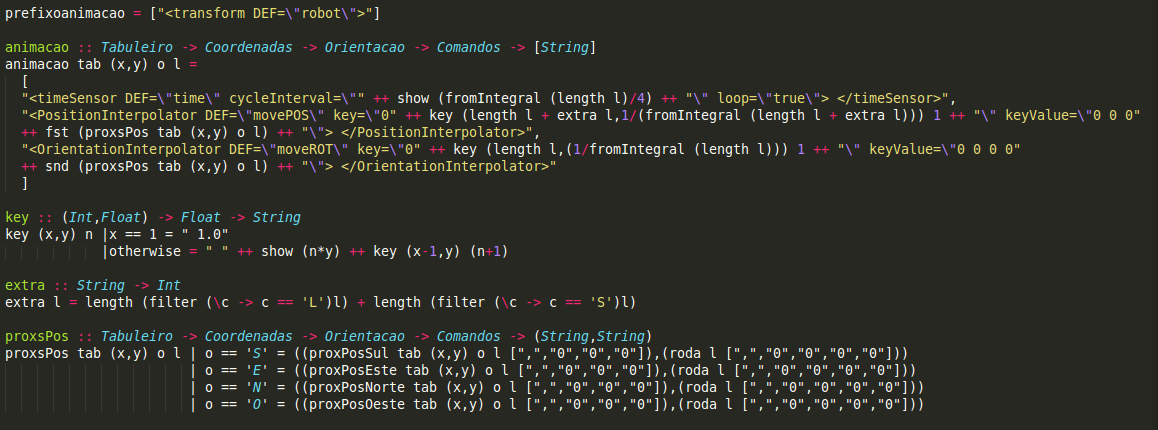
\includegraphics[scale=0.35]{./23.png}
 \textbf{\caption{Adaptações \textit{html} para possibilitarem a animação do \textit{robot}}}
\end{figure}
  


















\newpage

\item Como foi referido, a avaliação desta tarefa é essencialmente qualitativa, pelo que não é possível apontar a maior ou menor correção do programa da tarefa. Contudo, os testes do \textit{Mooshak} fazem uma verificação estrutural do código gerado pelo programa, com vista a perceber se este devolve ou não uma página \textit{html}. Nesse teste, o programa criado pelo grupo para esta quinta tarefa apresenta um "Presentation Error". 
\end{enumerate}

\section{Conclusão}

\begin{itemize}
    \item Em jeito de conclusão, diga-se que desfrutamos da criação deste jogo. Por um lado, pelo toque pessoal que lhe pudemos impor. Por outro, pela experiência que ele nos proporcionou, nomeadamente no que diz respeito ao contacto com a plataforma \LaTeX e o formato \textit{html}, sem nunca esquecer o aprofundar de conhecimentos nas aplicações \textit{Haskell}. 
\end{itemize}

\begin{figure}[b]
\centering

\includegraphics[scale=0.40]{./Picture2.png}
\end{figure}

\end{document}